% 2010 new curriculum science q4 fig1: circle x^2+y^2=4 with P0(sqrt2,-sqrt2) and P at +pi/4
\usetikzlibrary{arrows.meta,calc}
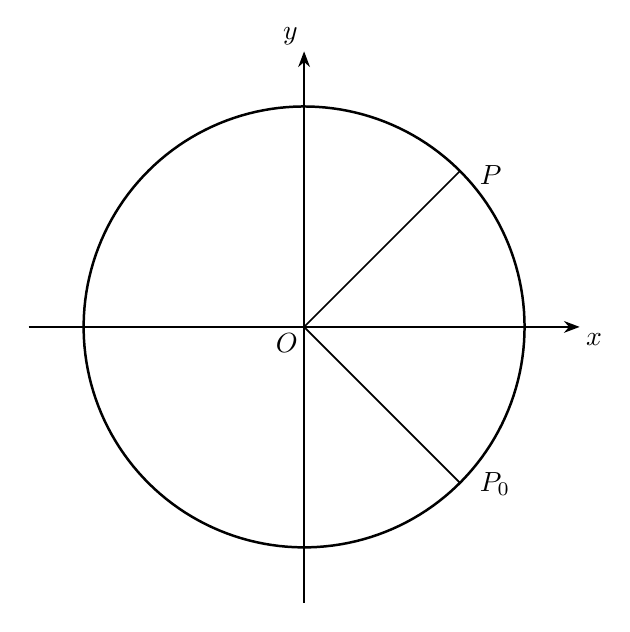
\begin{tikzpicture}[x=1.4cm,y=1.4cm,line width=0.6pt,>=Stealth]
\coordinate (O) at (0,0);
% axes
\draw[->] (-2.5,0) -- (2.5,0);
\node[below right=2pt,inner sep=0pt] at (2.5,0) {$x$};
\draw[->] (0,-2.5) -- (0,2.5);
\node[above left=2pt,inner sep=0pt] at (0,2.5) {$y$};
% circle
\draw[line width=0.9pt,domain=0:360,samples=180] plot ({2*cos(\x)},{2*sin(\x)});
% radii
\coordinate (P) at (1.414214,1.414214);
\coordinate (P0) at (1.414214,-1.414214);
\draw (O) -- (P);
\draw (O) -- (P0);
% labels
\node[anchor=north east,inner sep=0pt,xshift=-2pt,yshift=-2pt] at (O) {$O$};
\node[anchor=west] at ($(P)+(0.09,-0.04)$) {$P$};
\node[anchor=west] at ($(P0)+(0.09,-0.01)$) {$P_0$};
\end{tikzpicture}
